\subsection{Brugertilfredshed}

Et vigtigt element ved indførelse af ny teknologi er brugertilfredsheden, og denne har stor betydning for virkningen af den nye teknologi. En lav brugertilfredshed i forbindelse med anvendelse af aktivitetsarmbånd, vil resultere i lavere anvendelsesprocent, hvilket betyder teknologien ikke vil give lægen et fyldestgørende indblik i patientens aktivitetsmønster.

\subsubsection{Brugerbedømelse af Fitbit Flex}

For det valgte aktivitetsarmbånd, Fitbit Flex, er det fundet at armbåndet ikke scorer højest hvad angår tilfredsheden vedrørende egenskaber for armbåndet. I undersøgelsen 'A comparison of wearable fitness devices' har forsøgspersonerne anvendt hvert af armbåndene i en uge, hvorefter de er bedømt på en skala fra $1$ til $5$. Blandt fordele ved armbåndet, kan der blandt andet nævnes at forsøgspersonerne er tilfredse med det strømlinede design, at applikationens brugerflade er farverig, sjov og nem at bruge, samt at det er vandafvisende. Ulemperne inkludere blandt andet langsom synkronisering og problemer med tracking af gang på trapper \citep{kaewkannate2016}.

\begin{figure}[H]
	\centering
	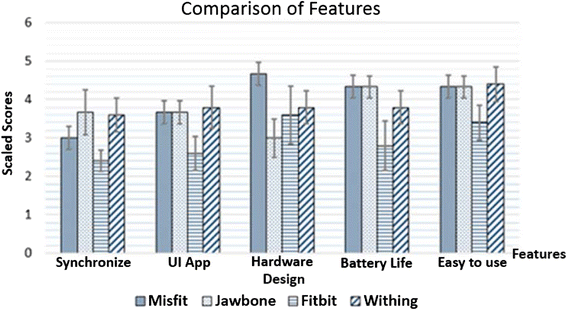
\includegraphics[width=0.6\textwidth]{figures/FeatureSatisfaction}
	\caption{Sammenligning af tilfredsheden vedrørende aktivitetsarmbåndenes egenskaber \citep{kaewkannate2016}.}
	\label{fig:FeatureSatisfaction}
\end{figure}

På \figref{fig:FeatureSatisfaction} ses det at Fitbit Flex's bedømmelse ligger omkring midten af tilfredsheds-skalaen anvendt i studiet 'A comparison of wearable fitness devices'. Dette betyder at brugerne finder armbåndet lettere anvendeligt og tilfredsstillende hvad angår synkronisering, brugerflade og batteritid, mens det bedømmes som moderat anvendeligt og tilfredsstillende vedrørende hardware design og brugervenlighed \citep{kaewkannate2016}.

\begin{figure}[H]
	\centering
	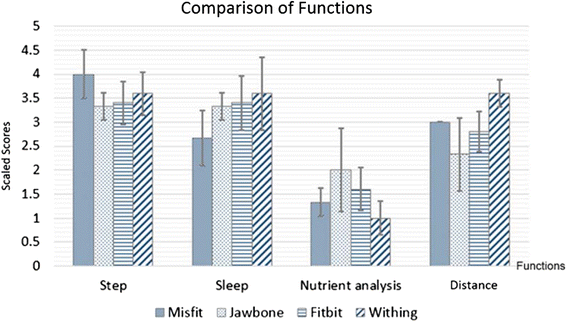
\includegraphics[width=0.6\textwidth]{figures/FunctionSatisfaction}
	\caption{Sammenligning af tilfredsheden vedrørende aktivitetsarmbåndenes funktioner \citep{kaewkannate2016}.}
	\label{fig:FunctionSatisfaction}
\end{figure}

Funktionaliteten er bedømt på \figref{fig:FunctionSatisfaction}, hvor det ses der ikke er en stor variation i brugernes bedømmelse af armbåndenes funktioner. Her er Fitbit Flex bedømt mellem lettere og moderat anvendeligt og tilfredsstillende ved optælling af skridt, søvnmåling og afstandsmåling. Alle armbånd er bedømt som meget lidt til lettere anvendeligt og tilfredsstillende i forbindelse med kostanalyse- og opmåling \citep{kaewkannate2016}.

\subsubsection{Anvendelse af aktivitetstracker i hverdagen}

For at opnå forståelse for patientens oplevelse ved brug af aktivitetstrackere i hverdagen, tages udgangspunkt i studierne 'Acceptance of Commercially Available Wearable Activity Trackers Among Adults Aged Over 50 and With Chronic Illness: A Mixed-Methods Evaluation' og 'Personal informatics for everyday life: How users without prior self-tracking experience engage with personal data'. Det førstnævnte studie undersøger implementeringen af aktivitetstrackere til motionsmonitorering af kronisk syge over 50 år, hvor forsøgspersonerne tester en simpel skridttæller og fire aktivitetstrackere, for til sidst at bedømme forskellige aspekter ved anvendelse af disse. I det andet studie undersøges hvordan forsøgspersoner uden tidligere erfaring med aktivitetstrackere oplever at måle deres aktivitetsniveau.


https://www.ncbi.nlm.nih.gov/pmc/articles/PMC3961803/ (Måske ikke så relevant)
https://www.ncbi.nlm.nih.gov/pmc/articles/PMC4749845/
http://www.sciencedirect.com/science/article/pii/S107158191630060X


\subsubsection{Motivation ved aktivitetstracking}

https://www.ncbi.nlm.nih.gov/pubmed/19902981
http://link.springer.com/article/10.1186/s13612-016-0042-6


Er teknologien brugervenlig og motiverer den patienten til en mere aktiv hverdag?

Er aktivitetsarmbåndet brugervenligt/let at anvende/lære at anvende?

Hvad kræver det af patienten at anvende aktivitetsarmbåndet?